\chapter{不純物を含まないクリーンな系における強結合理論}\label{sec:append:pure}

\s{絶対零度における BCS-Leggett 理論}\label{sec:append:pure:bcsl}

不純物が存在しないクリーンな系では、式 (\ref{eq:form:mnf:gapeq}) と (\ref{eq:form:mnf:numeq}) は次のようになる。
\beq
&\frac{m}{4 \pi \as} + \sum_{\bp}\left[ \frac{1}{\beta}\sumn\frac{1}{\omn^2+\del^2 + (\ken_{\bp}-\cpt)^2} - \frac{1}{2 \ken_{\bp}}\right] = 0,\label{eq:append:matsu:del}\\
&N = \sum_{\bp} \left[ 1 - \frac{2}{\beta}\sum_n \frac{ \ken_{\bp} - \cpt}{\omn^2+\del^2+(\ken_{\bp}-\cpt)^2} \right].\label{eq:append:matsu:num}
\eeq
松原周波数の和は計算することができて、後者は、
\beq
 \frac{1}{\beta}\sumn\frac{1}{\omn^2+\del^2 + (\ken_{\bp}-\cpt)^2}=  \frac{\tanh \frac{ \beta E_p}{2}}{2E_p}.\label{eq:append:matsu:int}
 \eeq
ここで $E_p = \sqrt{\del^2 + (\ken_p-\cpt)^2}$ は超流動状態における 1 粒子励起スペクトルを表す。


\begin{figure}[t]
\centering
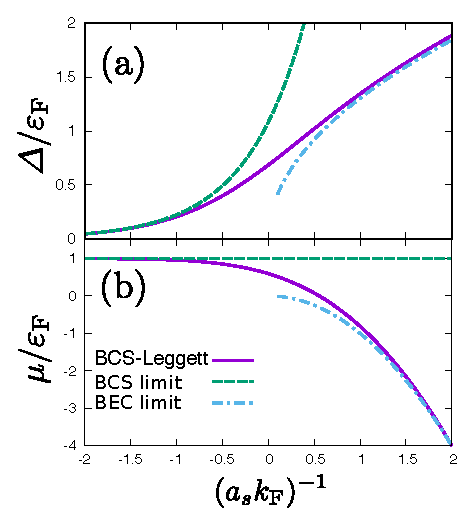
\includegraphics[width=80mm]{eps/pure-bcsl.eps}
\caption{BCS-Leggett 理論で得られたクリーンな系の (a)超流動秩序変数 $\del$、 と (b)化学ポテンシャル $\cpt$。実線はBCS-Leggett 理論による結果。破線は BCS 極限の結果で $\del$ は式 (\ref{eq:append:pure:limitbcs})、$\cpt$ は $\eqf$ で与えられる。点破線は BEC 極限の結果で $\del$ は式 (\ref{eq:append:pure:limitbec-del})、$\cpt$ は式 (\ref{eq:append:pure:limitbec-cpt}) で与えられる。}
\label{fig:bcsl:pure:bcsl}
\end{figure}

式 (\ref{eq:append:matsu:int}) を用いれば、式 (\ref{eq:append:matsu:del})、(\ref{eq:append:matsu:num}) は、
\beq
&\frac{m}{4 \pi a_s} + \sum_{\bp} \left[\frac{\tanh \frac{ \beta E_p}{2}}{2E_p}  - \frac{1}{2 \ken_{\bp}} \right] = 0,\label{eq:append:pure:del}\\
&N = \sum_{\bp} \left[ 1 - \frac{\ken_{\bp} - \cpt}{ E_p}\tanh \frac{\beta E_p}{2}\right].\label{eq:append:pure:num}
\eeq
特に $T=0$ においては $E_p>0$ に注意して、
\beq
&\frac{m}{4 \pi a_s} + \sum_{\bp} \left[\frac{ 1}{ 2 E_p} - \frac{1}{2 \ken_{\bp}} \right],\label{eq:append:pure:del2}\\
&N = \sum_{\bp}\left[1- \frac{\ken_{\bp}-\cpt}{2E_{\bp}}\right],\label{eq:append:pure:num2}
\eeq
となる。

弱結合 BCS 極限では $\cpt=\eqf$ であり、また $\del\ll \eqf$ に注意すると、式 (\ref{eq:append:pure:del2}) から、
\beq
\varDelta = 8 e^{\frac{\pi}{2 \askf} - 2} \eqf, \label{eq:append:pure:limitbcs}
\eeq
を得る。

一方で、強結合 BEC 極限 $\askfi \to \infty$ では、式 (\ref{eq:append:pure:del2}) より、
\beq
\cpt = - \frac{1}{(\askf)^2} \eqf, \label{eq:append:pure:limitbec-cpt}
\eeq
が得られるが、これは 2 体束縛状態の結合エネルギーの半分の大きさに等しい。これを式 (\ref{eq:append:pure:num2}) に代入すると、
\beq
\del = \sqrt{\frac{16}{3 \pi}} |\cpt|^{1/4} \eqf^{3/4}, \label{eq:append:pure:limitbec-del}
\eeq
が得られる。

図 \ref{fig:bcsl:pure:bcsl} には、BCS-Leggett 理論の方程式 (\ref{eq:append:pure:del2}), (\ref{eq:append:pure:num2}) を自己無撞着に解いて得られた $\del$ と $\cpt$、および BCS極限、BEC 極限の結果をまとめてある。


\s{不純物がない場合の $T$ 行列近似(正常相:$T\ge \tc$)} \label{sec:append:pure:tma}
 
ここでは、不純物を含まないフェルミ原子気体に対する通常の $T$ 行列近似の表式をまとめる。

式 (\ref{eq:form:tma:sigpom}) から式 (\ref{eq:form:tma:piimp}) において、$c=0$(つまり不純物なし)とすることは、$\gimppom$ を $\gzrpom$ に、$\vtxp$ を $1$ に置き換えることに対応する。すると、
\beq
\left[\gpom\right]^{-1} &= \left[ \gzrpom\right]^{-1} - \sigpom,\label{eq:append:tma:g}\\
\sigpom &= \frac{1}{\beta} \sumn \sum_{\bq} \gamqnu \gzrqnu,\label{eq:append:tma:sig}\\
\gamqnu &= \frac{-U}{1-U\piqnu},\label{eq:append:tma:gam}\\
\piqnu &= \frac{1}{\beta} \sumn \sum_{\bp} \gzrpom \gzrqnu.\label{eq:append:tma:pi}
\eeq

実際、これはクリーンな系のフェルミ原子気体の BCS-BEC クロスオーバー領域の研究で用いられる $T$ 行列近似の表式に一致する \cite{ohashi2005}。

\begin{figure}[t]
\centering
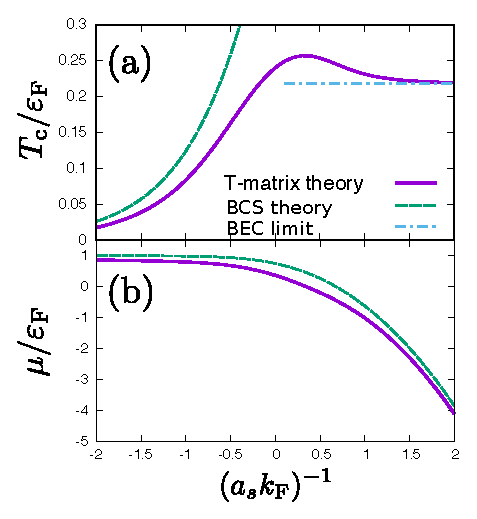
\includegraphics[width=80mm]{eps/pure-tma.eps}
\caption{$T$ 行列近似で得られた、不純物を含まないフェルミ原子気体の BCS-BEC クロスオーバー領域における (a)超流動転移温度 $\tc$ と (b)化学ポテンシャル $\cpt(T=\tc)$ }
\label{fig:bcsl:pure:tma}
\end{figure}


式 (\ref{eq:append:tma:pi}) の松原周波数の和はクリーンな系では実行することができ、
\beq
\piqnu &= - \frac{1}{2}\sum_{\bp} \left[\frac{\tanh\frac{\beta\left[\ken_{\bp+\bqt}-\cpt\right]}{2}+\tanh\frac{\beta\left[\ken_{\bp-\bqt}-\cpt\right]}{2}}{i\num -2 (\ken_{p}+\ken_{q/2} -  \mu)}\right].\label{eq:append:tma:pii}
\eeq
ここで式 (\ref{eq:append:tma:pii}) では $\bp\to \bp+\bqt$ と取り直した。式 (\ref{eq:append:tma:pii}) を用いると、サウレスの判定条件は、式 (\ref{eq:append:tma:gam}) の分母を $\bq=0$, $i\num=0$ に対し 0 として、
\beq
1&=U \varPi_{\bq=0}(i\num=0) \notag\\
&= -\frac{4\pi a_s}{m}\sum_{\bp} \left[ \frac{\tanh\frac{\beta \left[\ken_{\bp}-\cpt\right]}{2}}{2(\ken_{\bp} -  \cpt)}- \frac{1}{2 \ken_p} \right].\label{eq:append:tma:tcdet}
\eeq
これは、式 (\ref{eq:append:pure:del}) のギャップ方程式で $\del=0$ としたものと一致する。粒子数方程式は、式 (\ref{eq:append:tma:g}) を式 (\ref{eq:form:tma:number}) に用いることで得られる。こうして得られた $\tc$ の方程式 (\ref{eq:append:tma:tcdet}) と粒子数方程式から $\tc$ と $\cpt$ を自己無撞着に決定して得られたものが図 \ref{fig:bcsl:pure:tma} である。

平均場 BCS 理論は、粒子数方程式 (\ref{eq:append:tma:g}) でグリーン関数 $\gpom$ を自由フェルミ気体のそれに置き換えたもの、
\beq
\gpom \Rightarrow \gzrpom = \frac{1}{i \omn - (\ken_p-\cpt)},
\eeq
と、サウレスの判定条件 (\ref{eq:append:tma:tcdet}) で構成される。通常、弱結合 BCS 領域を考える場合は更に $\cpt = \eqf$ とし、粒子数方程式は扱わずにギャップ方程式 (\ref{eq:append:tma:tcdet}) のみを扱う。

強結合 BEC 極限は $\tc$ 以上ですでに形成された分子ボソンの BEC として超流動転移が記述される。今、全てのフェルミ原子が $N/2$ 個の分子を形成しているとすると、この理想分子ボース気体の BEC 転移温度は分子ボソンの運動エネルギーを $E_q\equiv q^2/(2M)$ と書いて、
\beq
\frac{N}{2}& =\frac{k_{\text{F}}^3}{6\pi^2} = \sum_q \frac{1}{e^{\beta E_q}-1} = \frac{k_{\text{F}}^3}{4 \pi^2} \left[ 2 \frac{T_{\text{BEC}}}{\eqf}\right]^{3/2}\zeta(3/2) \varGamma(3/2),
\eeq
よりもとまる。これを $T_{\text{BEC}}$ に対して解くと、
\beq
T_{\text{BEC}} = \frac{1}{2} \left[\frac{2}{3 \zeta\left(\frac{3}{2}\right) \varGamma\left(\frac{3}{2}\right)}\right]^{3/2} \eqf \simeq 0.218 \eqf,\label{eq:append:tma:bose}
\eeq
を得る。図 \ref{fig:bcsl:pure:tma} に示すように $T$ 行列近似で計算された $\tc$ は、$\askfi \to \infty$ の BEC 極限で式 (\ref{eq:append:tma:bose}) で与えられる $T_{\text{BEC}}$ に漸近する。




\chapter{アンダーソンの定理}\label{sec:append:anderson}

粒子-ホール対称性を課し、運動量積分をエネルギー積分に変換した際、1 粒子状態密度のエネルギー依存性を無視してフェルミ面での値で近似すると、
\beq
\sum_{\bp}\frac{ (\ken_{\bp} - \tcptn) \tau_3}{\tomn^2 + \tdeln^2 + (\ken_{\bp}-\tcptn)^2}&\simeq \fdos \int^{\infty}_{-\infty} \diff \ken \frac{(\ken + \cpt- \tcptn) \tau_3}{\tomn^2 + \tdeln^2 + (\ken+\cpt-\tcptn)^2}\notag\\
&= \fdos \int^{\infty}_{-\infty} \diff \ken \frac{\ken \tau_3}{\tomn^2 + \tdeln^2 + \ken^2}  = 0,
\eeq
となり、化学ポテンシャルシフトの松原周波数依存性がなくなる。ここでフェルミエネルギーは十分大きいとして、エネルギー積分の下限を $-\infty$ とした。この時、式 (\ref{eq:form:mnf:gapeq}) は、$\tcptn = \cpt$ として、
\beq
\frac{m}{4 \pi \as} + \sum_{\bp}\left[ \frac{1}{\beta}\sumn \frac{ \tdeln}{\del} \frac{1}{\tomn^2+\tdeln^2 + (\ken_{\bp}-\cpt)^2} - \frac{1}{2 \ken_{\bp}}\right] = 0,
\eeq
となる。さらに、
\beq
\sum_{\bp} \frac{ \tdeln}{\del} \frac{1}{\tomn^2+\tdeln^2 + (\ken_{\bpp}-\cpt)^2} & = \fdos \int^{\infty}_{-\infty} \diff \ken \frac{ \tdeln}{\del} \frac{1}{\tomn^2+\tdeln^2 + \ken^2} \notag\\
&= \fdos \frac{ \tdeln}{\del} \frac{\pi}{\sqrt{\tomn^2+\tdeln^2 }},
\eeq
および式 (\ref{eq:form:mnf:nonmag}) の等式 $\omn/\omega=\tdeln/\del$ を用いれば、
\beq
\frac{m}{4 \pi \as} +\frac{1}{\beta}\sumn \frac{1}{\sqrt{\omega^2+\del^2}}-\sum_{\bp}\frac{1}{2 \ken_{\bp}}= 0.\label{eq:append:mnf:gapgap}
\eeq
式 (\ref{eq:append:mnf:gapgap}) は、非磁性不純物を含まない場合のギャップ方程式に一致する。よってこの場合、非磁性不純物散乱は超流動秩序パラメータに影響を与えない(アンダーソンの定理)。



\chapter{超流動転移温度以下の不純物 $T$ 行列理論}\label{sec:append:imptmasf}

ここでは \ref{sec:form:tmat} 節で説明した超流動転移温度以上の $T$ 行列理論を超流動状態に拡張する方法を説明する。\ref{sec:append:outoukansu} 節でまず、\ref{sec:form:bcsl} 節で定式化した非磁性不純物を含む BCS-Leggett 理論で記述される超流動状態に対し、超流動ゆらぎを加えた場合の対波動関数応答を線形応答で調べる。\ref{sec:append:outoukansudiagram} 節は、その応答関数を与えるダイアグラムを説明する。\ref{sec:append:outouttmat} 節でこのダイアグラムを自己エネルギーに取り込むことで、非磁性不純物を含む有限温度の $T$ 行列理論を構成する。最後に \ref{sec:append:rewritetmat} 節で、\ref{sec:form:tmat} 節で説明した超流動転移温度以上での理論にどうつながるか説明する。


\section{超流動揺らぎに対する対波動関数の応答関数}\label{sec:append:outoukansu}
非磁性不純物を含む系において、どのようなダイアグラムが超流動揺らぎに寄与するかを調べるために、超流動転移温度以下において、超流動揺らぎに対する対波動関数の応答関数を考える。超流動揺らぎを引き起こす外場として、対振幅 $\varPhi_{\bq}=\braket{\rho_-(-\bq)}$, $\varPhi_{\bq}^{\ast}=\braket{\rho_+(\bq)}$ を時刻 $t_0\to-\infty$ から印可することを考える。すなわち、次のように仮想的な外場を摂動として系に加える。
\beq
F_{\bq}(t)&=\sum_{\bp}\braket{c_{-\bp+\bqt,\dar} c_{\bp+\bqt,\dar}}\theta(t-t_0) = \varPhi_{\bq}\theta(t-t_0),\\
F_{\bq}^{\ast}(t)&=\sum_{\bp}\braket{c_{\bp+\bqt,\dar}^{\dag}c_{-\bp+\bqt,\dar}^{\dag} }\theta(t-t_0) =\varPhi_{\bq}^{\ast}\theta(t-t_0).
\eeq
ここで $\rho_{\pm}(\bm{q})=\sum_{\bp} \varPsi_{\bp+\bqt}^{\dag} \tau_{\pm} \varPsi_{\bp-\bqt}$ であり、$\theta(t)$ は階段関数である。この時、摂動ハミルトニアンは、
\beq
\hanah'(t) &= -U \sum_{\bq} \left[ \rho_+ (\bq) F_{\bq}(t) + F^{\ast}_{\bq}(t) \rho_-(-\bq)\right],\label{eq:append:ham:ext}
\eeq
となる。式 (\ref{eq:append:ham:ext}) による対波動関数 $\varPhi_{\bq}=\braket{\rho_-(-\bq)}$, $\varPhi_{\bq}^{\ast}=\braket{\rho_+(\bq)}$  の線形応答を調べると、
\beq
&\delta \varPhi_{\bq} (t)=-i \int^{\infty}_{\infty} \diff t' \Tr \left\{\rho_{\text{eq}} \left[\hanah'(t),\rho_-(-\bq,t)\right]\right\}\notag\\
&\qquad =iU  \int^{\infty}_{-\infty} \diff t'\left[\braket{\left[\rho_+(\bm{q},t'), \rho_-(-\bq,t)\right]}_{\text{eq}} F_{\bq}(t')+\braket{\left[\rho_-(-\bm{q},t'), \rho_-(-\bq,t)\right]}_{\text{eq}} F_{\bq}^{\ast}(t')\right]\notag\\
&\qquad \equiv -U \int^{\infty}_{-\infty}\diff t'  \left[\chi_{-+}(\bq,t-t') F(t') + \chi_{--}(\bq,t-t')F_{\bq}^{\ast}(t')\right].\label{eq:append:below:deltaphi}
\eeq
となる。時間に関し、フーリエ変換すると、
\beq
\delta \varPhi_{\bq}(\omega) = - U \chi_{-+}(\bq, \omega) F_{\bq}(\omega) - U \chi_{--}(\bq,\omega) F^{\ast}_{\bq}(\omega).
\eeq
ここで、
\beq
\chi_{-\pm}(\bq,\omega) = \int^{\infty}_{-\infty} \diff t\ \chi_{-\pm}(\bq,t) e^{i \omega t}.
\eeq
$\delta \varPhi_{\bq}^{\ast}(\omega)$ に対しても同様の計算を行い、式 (\ref{eq:append:below:deltaphi}) のように $\chi_{+-}(\bq,\omega)$, $\chi_{++} (\bq,\omega)$ を導入すると、
\beq
\begin{pmatrix}
\delta \varPhi_{\bq}^{\ast}(\omega) \\ \delta \varPhi_{\bq}(\omega)
\end{pmatrix}
= -U
\begin{pmatrix}
\chi_{+-}(\bq,\omega) & \chi_{++}(\bq,\omega) \\
\chi_{--}(\bq,\omega) & \chi_{-+}(\bq,\omega) 
\end{pmatrix}
\begin{pmatrix}
F_{\bq}^{\ast}(\omega) \\ F_{\bq}(\omega)
\end{pmatrix}, \label{eq:append:below:deltaqom}
\eeq
を得る。式 (\ref{eq:append:below:deltaqom})で定義した $\chi_{\pm\pm}$ は、Nambu 場で表された 2 体の遅延グリーン関数であり、ダイアグラム法で計算できる虚時間形式で計算した後、それを解析接続をすることで求めることができる。対応する虚時間形式の相関関数は、
\beq
\chi_{\pm\pm} (\bq, \tau) = - \braket{T_{\tau} \left\{ \rho_{\pm}(\pm\bq, \tau) \rho_{\pm}(\pm\bq,0)\right\} }
\eeq
のフーリエ変換、
\beq
\chi_{\pm\pm}(\bq,i \num) = \int^{\beta}_0 \diff \tau \chi_{\pm\pm} ( \bq, \tau) e^{i \num \tau},
\eeq
で与えられる。

\section{応答関数のダイアグラム展開}\label{sec:append:outoukansudiagram}

\ref{sec:append:outoukansu} 節で考えた $\chi_{\pm\pm}(\bq, i \num)$ を、 1 粒子温度グリーン関数とコンシステントになるような近似を行うことが重要である。これはワード高橋恒等式を満たすよう理論を構成することに等しい \cite{schrieffer1983}。

\begin{figure}[t]
\begin{center}
\includegraphics[width=100mm]{eps/belowtc-vtx-full.eps}
\end{center}
\caption{非磁性不純物を含む BCS-Leggett 理論の自己エネルギー(式 (\ref{eq:form:mnf:sig}))とコンシステントな 3 点バーテックス $\widetilde{\varGamma}$。2本線は非磁性不純物 BCS-Leggett 理論で求まるグリーン関数 $\bgimppom$ を表す。右辺第一項はグリーン関数に外場を直接挿入した裸のバーテックスであり、$\tau_{\pm}$ で表される。右辺第二項は不純物散乱によるの自己エネルギー中の全てのグリーン関数に外場を挿入することで得られるもので、$\times$ 印は不純物濃度 $c$、黒三角形は BCS-Leggett 理論で用いた黒三角形と同じ $\vvtxn$ である。右辺最終項は原子間相互作用のダイアグラム中の 1 粒子グリーン関数に外場を挿入することで得られる 3 点バーテックスである。}
\label{fig:below:vtx:full}
\end{figure}


無摂動状態として、図 \ref{fig:form:mnf:sigimp} に示した非磁性不純物を含む BCS-Leggett 理論で記述される状態を考える。この時、平均場理論の自己エネルギー(式 (\ref{eq:form:mnf:sig}))中の 1 粒子グリーン関数の全てに外場のダイアグラムを“差し込んで”得られる 3 点バーテックス $\widetilde{\varGamma}$ を用いることでワード高橋恒等式を満たすことができる。これを行うと $\widetilde{\varGamma}$ は、図 \ref{fig:below:vtx:full} のダイアグラムで与えられる。式 (\ref{eq:append:ham:ext}) で与えられる摂動ハミルトニアンを平均場の自己エネルギーに挿入するので、その部分には $\tau_{\pm}$ の行列要素が付与される。また、図 \ref{fig:below:vtx:full} 中の $\vvtxn$ は、
\beq
\vvtxn = \frac{1}{\frac{m}{2 \pi \bs} \tau_3 - \sum_{\bpp}\left[ \bgimpppom +  \frac{\tau_3}{\ken_{\bpp}}\right]},\label{eq:asdfasdfasdfasdf}
\eeq
で与えられる。

\newcommand{\tsom}{T^{s}_{\bq}(i\omn,i\omn+i\num)}
\begin{figure}[t]
\begin{center}
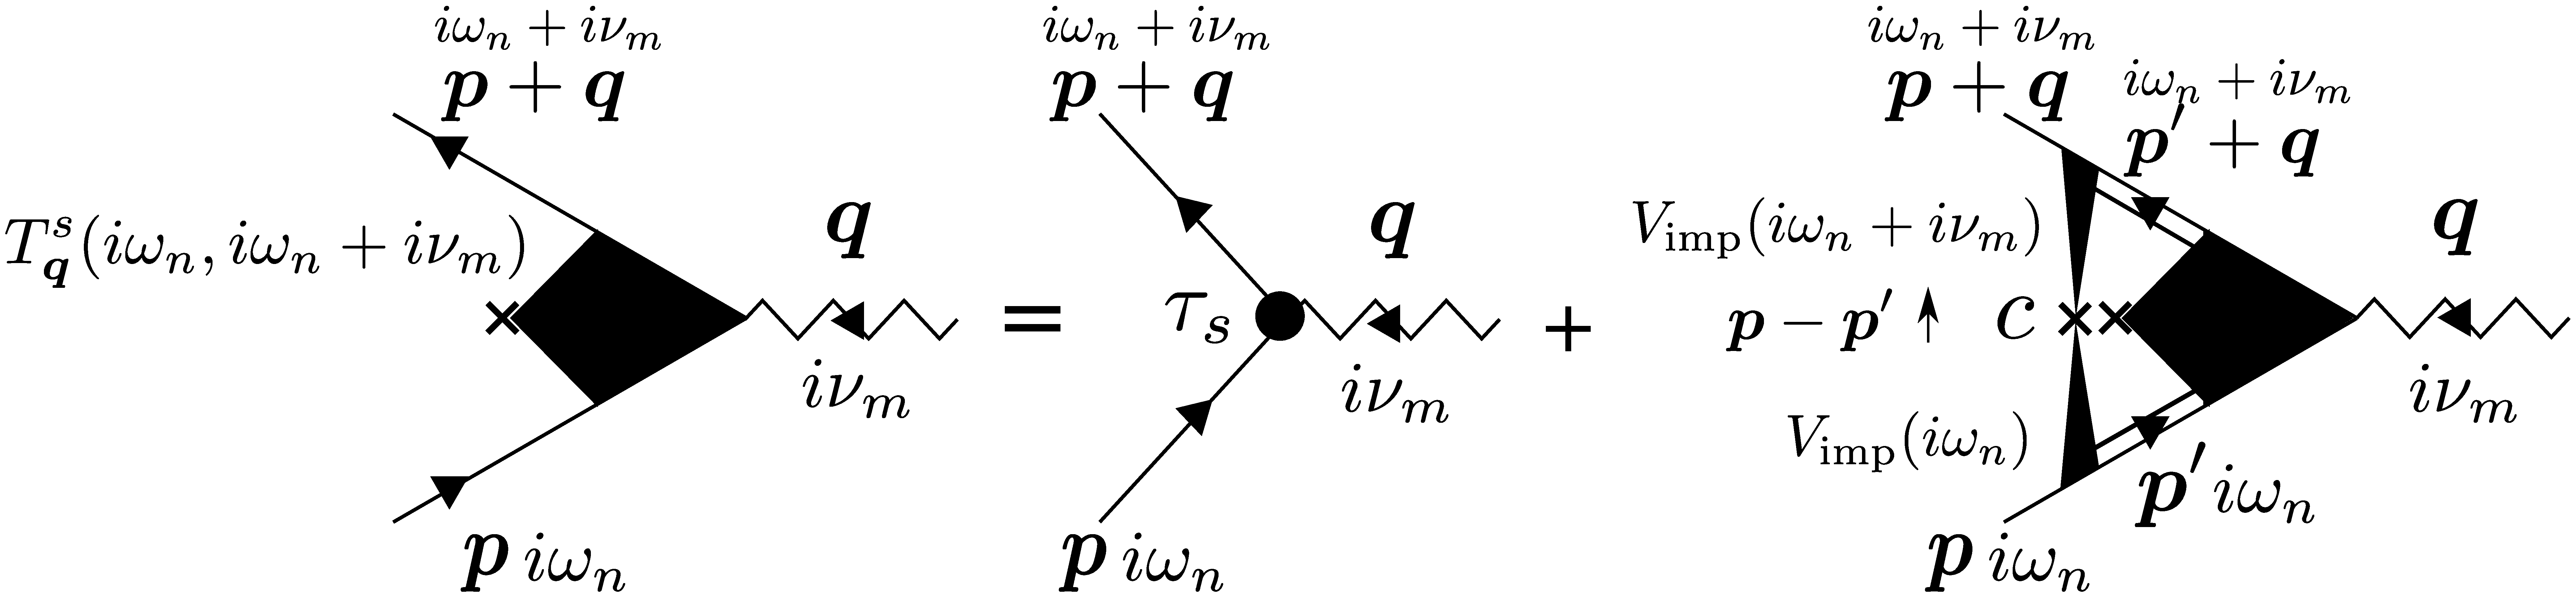
\includegraphics[width=120mm]{eps/belowtc-vtx-imp.eps}
\end{center}
\caption{非磁性不純物散乱のみを考慮した 3 点バーテックス $\tsom$ のファインマンダイアグラム。}
\label{fig:below:vtx:imp} 
\end{figure}


この 3 点バーテックス $\widetilde{\varGamma}$ を計算するために、まず図 \ref{fig:below:vtx:imp} のように散乱前後で松原周波数を変化させない不純物散乱に因るバーテックス補正のみを足しあげる。これを $\tsom$ と書くと、
\beq
\tsom &= \tau_s\notag\\
& + c \sum_{\bpp} \vvtxn \bgimpppom \tsom \notag\\
& \times \bgimp_{\bpp+\bq}(i\omn+i\num) \vvtx (i\omn+i\num).\label{eq:append:tma:tsom}
\eeq

この式 (\ref{eq:append:tma:tsom}) は $\tsom$ について解くことができる。そのために以下の手順に従って、$2 \times 2 $ 行列を $4\times 4$  行列へと書き換え、右辺第二項の $\tsom$ を 4 成分ベクトルに書き換えたものに、左からのみ行列がかかるように書き換える。まず
\beq
A_{2 \times 2} = \begin{pmatrix} a_{11} & a_{12} \\ a_{21} & a_{22} \end{pmatrix},
\eeq
とかける $2 \times 2$ 行列に対し、$A_{2 \times 2}$ が $\tsom$ へ左から演算される場合には、
\beq
A_{2 \times 2} \longleftrightarrow A_{4\times 4}^{(\text{L})} \equiv A_{2\times 2} \otimes \bm{1} ={\tiny \begin{pmatrix} a_{11} &0&a_{12}& 0\\0&a_{11} & 0 & a_{12} \\ a_{21} & 0 & a_{22}& 0 \\ 0& a_{21}& 0 &a_{22}\end{pmatrix}},\label{eq:a22toal44}
\eeq
のように $4 \times 4$ 行列 $A_{4 \times 4}^{(\text{L})}$ へと書き換える。次に、$A_{2 \times 2}$ が $\tsom$ に右から演算する場合には、
\beq
A_{2 \times 2} \longleftrightarrow A_{4\times 4}^{(\text{R})} \equiv \bm{1} \otimes A_{2\times 2}^{T} = {\tiny \begin{pmatrix} a_{11} &a_{21}&0 &0  \\ a_{12} & a_{22}& 0 & 0 \\ 0&0&a_{11}&a_{21} \\ 0&0&a_{12}&a_{22}\end{pmatrix}},\label{eq:a22toar44}
\eeq
と $4 \times 4$ 行列 $A_{4 \times 4}^{(\text{R})}$ へと書き換えて、$\tsom$ に対して左から演算させる。また、$T^s$ そのものは 4 成分ベクトルへと書き換えは以下のように行う。$2 \times 2$ 行列 $B_{2 \times 2}$ と $4$ 次元ベクトル $B_4$ の対応づけは、2 つの 2 次元ベクトル $z^{T}=(z_1, z_2)$, $w^{T}=(w_1, w_2)$ を用いて、
\beq
B_{2 \times 2}= z \otimes w^T = \begin{pmatrix} z_1w_1 & z_1 w_2 \\ z_2 w_1 & z_2 w_2\end{pmatrix} \longleftrightarrow B_{4}=z\otimes w =\begin{pmatrix}z_1 w_1\\z_1w_2\\z_2w_1\\z_2w_2\end{pmatrix},\label{eq:b22tob4}
\eeq
と書き換える。式 (\ref{eq:a22toal44}), (\ref{eq:a22toar44}), (\ref{eq:b22tob4}) から、
\beq
&A^1_{2\times2} A^2_{2 \times 2} \cdots A^n_{2 \times 2} B_{2 \times 2 } C^{1}_{2 \times 2} C^2_{2 \times 2} \cdots C^{m}_{2 \times 2}\notag\\
&\quad \longleftrightarrow A^{1 (L)}_{4 \times 4}A^{2 (L)}_{4 \times 4} \cdots A^{n (L)}_{4 \times 4}C^{m (R)}_{4 \times 4}\cdots C^{2 (R)}_{4 \times 4} A^{1 (R)}_{4 \times 4} B_{4},\label{eq:rewritingssss}
\eeq
という書き換えができる。

式 (\ref{eq:append:tma:tsom}) は、式 (\ref{eq:rewritingssss}) の書き換えを、$\tsom \leftrightarrow B_{2 \times2 }$ として用いることで、次のように $\tsom$ について解くことができる。
\beq
&\left[ T^{s}_{\bq}(i \omn, i \omn+i\num)\right]_{4} = \left[\vphantom{ \sum_{\bpp} } 1-c \left[\vvtxn \right]^{(\text{L})}_{4\times 4} \left[V_{\imp}(i\omn+i \num) \right]^{(\text{R})}_{4\times4} \right.\notag\\
&\qquad \left. \times \sum_{\bpp} \left[\bgimp_{\bpp}(i\omn+i \num) \right]^{(\text{L})}_{4\times 4}  \left[\bgimp_{\bpp+\bq}(i\omn+i \num) \right]^{(\text{R})}_{4\times 4} \right]^{-1} \left[ \tau_s\right]_4.\label{eq:append:asdfasdfasdf}
\eeq



\begin{figure}[t]
\begin{center}
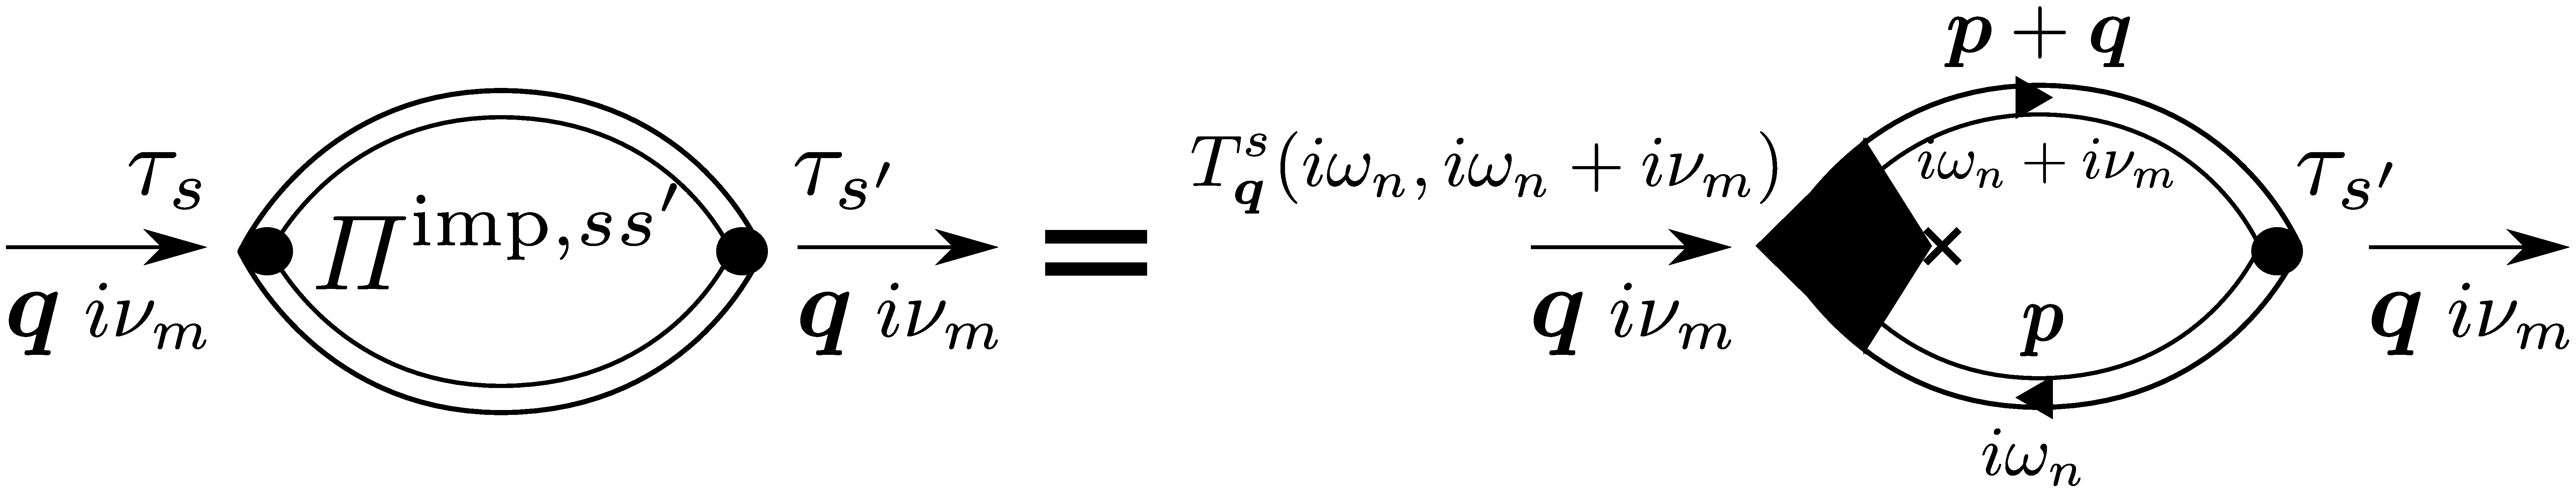
\includegraphics[width=100mm]{eps/belowtc-pi-imp.eps}
\end{center}
\caption{不純物散乱による補正を受けた対相関関数 $\varPi^{\imp, ss'}(i\num)$。黒四角は図 \ref{fig:below:vtx:imp} で示した不純物による 3 点バーテックス $\tsom$。}
\label{fig:below:pi:ppp}
\end{figure}

\begin{figure}[t]
\begin{center}
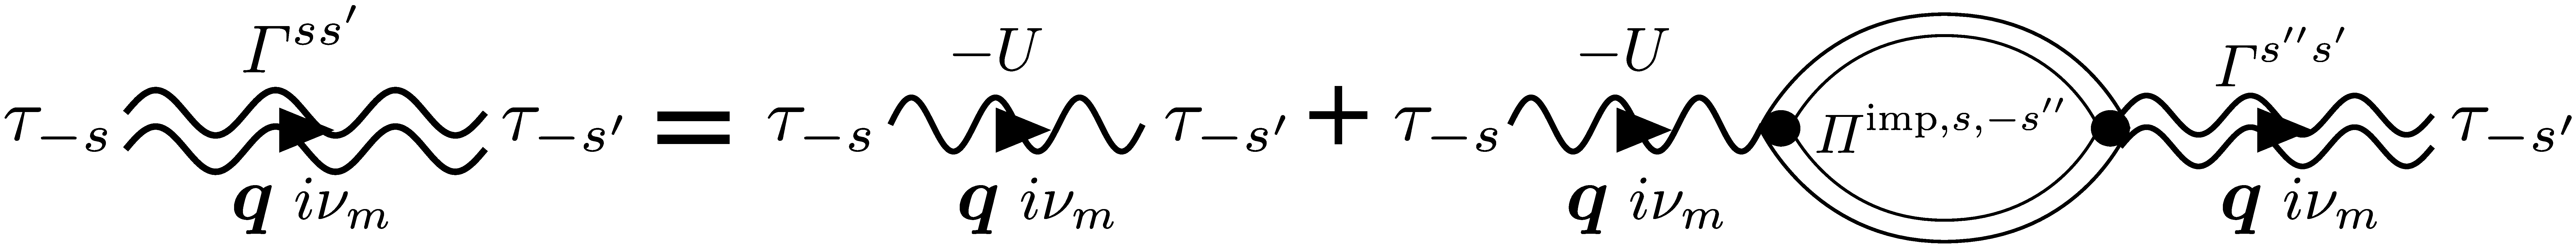
\includegraphics[width=120mm]{eps/belowtc-gam-dyson.eps}
\end{center}
\caption{原子間相互作用に対する補正を表す $\varGamma^{ss'}_{\bq}(i\num)$。図 \ref{fig:below:vtx:full} の 3 点バーテックス $\widetilde{\varGamma}$ において、原子間相互作用部分を解くために用いる。}
\label{fig:below:gam:ppp}
\end{figure}

次に原子間相互作用によるバーテックス補正を考える。図 \ref{fig:below:pi:ppp} のように不純物による頂点補正を繰り込んだ南部場のループを $\varPi^{\text{imp},ss'}_{\bq}(i\num)$ ($s, s'=\pm$)とすると、
\beq
&\varPi^{\text{imp},ss'}_{\bq}(i\num) \notag\\
&\qquad = \frac{1}{\beta}\sum_{i \omega_n}\sum_{\bp}\Tr \left[ \tsom \bgimp_{\bp+\bq}(i\omn+i\num) \tau_{s'}  \bgimppom \right], \label{eq:varpispaidf}
\eeq 
となる。この $\varPi^{\text{imp},ss'}$ を用いて、フェルミオン間相互作用の散乱行列 $\varGamma^{s,s'}_{\bq}(i \num)$ は、図 \ref{fig:below:gam:ppp} より、
\beq
&\varGamma^{s,s'}_{\bq}(i \num) = -U \delta_{s, -s'} -U\varPi^{\text{imp},ss''}_{\bq}(i\num) \varGamma^{-s'',s'}_{\bq}(i\num),\label{eq:append:asdfjjjjjjj}
\eeq
となる。これより、
\beq
\begin{pmatrix}
\varGamma^{+-}_{\bq}(i\num) &\varGamma^{++}_{\bq}(i\num)\\
\varGamma^{--}_{\bq}(i\num) &\varGamma^{-+}_{\bq}(i\num)
\end{pmatrix}^{-1}
= 
-\frac{1}{U} 
-
\begin{pmatrix}
\varPi^{\imp,+-}_{\bq}(i\num) & \varPi^{\imp,++}_{\bq}(i\num) \\
\varPi^{\imp,--}_{\bq}(i\num) & \varPi^{\imp,-+}_{\bq}(i\num)
\end{pmatrix},\label{eq:append:gam:gam}
\eeq
を得る。以上から $\widetilde{\varGamma}_{\bq}^{s}(i \omn, i \omn+i\num)$ は、
\beq
&\widetilde{\varGamma}_{\bq}^{s}(i \omn, i \omn+i\num) = \tsom +  \sum_{s',s''=\pm}T_{\bq}^{s'}(i \omn, i \omn+i\num) \varGamma^{-s',-s''}_{-\bq}(-i\num) \notag\\
&\qquad \times \frac{1}{\beta}\sum_{i \omega_n'}\sum_{\bpp}\Tr \left[ T^{s''}_{-\bq}(i\omn'+i\num,i\omn') \bgimppomp \widetilde{\varGamma}_{\bq}^{s}(i\num)  \bgimp_{\bpp+\bq}(i\omn'+i\num) \right].
\eeq
これを用いると、超流動ゆらぎを表す対相関関数 $\chi_{ss'} (\bq, i\num)$ は次のようになる。
\beq
\chi_{ss'} (\bq, i\num) =\frac{1}{\beta} \sumn \sum_{\bp} \Tr \left[\tau_{s} \bgimppom \widetilde{\varGamma}_{\bq}^{s'}(i \omn, i \omn+i\num)  \bgimp_{\bp+\bq}(i\omn+i\num)\right]
.\eeq

\section{超流動状態におけるの非磁性不純物が存在する場合の $T$ 行列理論}\label{sec:append:outouttmat}

\ref{sec:form:bcsl} 節の非磁性不純物含む BCS-Leggett 理論のグリーン関数、
\beq
\bgimppom = \frac{1}{i \tomn - \left[ \ken_{\bp} - \tcptn\right] \tau_3 + \tdeln \tau_1},\label{eq:thissection:f:f}
\eeq
は式 (\ref{eq:form:ham:abcslimp}), (\ref{eq:form:mnf:gimpopmpom}) を解くことで決定される。このグリーン関数 $\bgimppom$ を無摂動のグリーン関数とする。


\begin{figure}[t]
\begin{center}
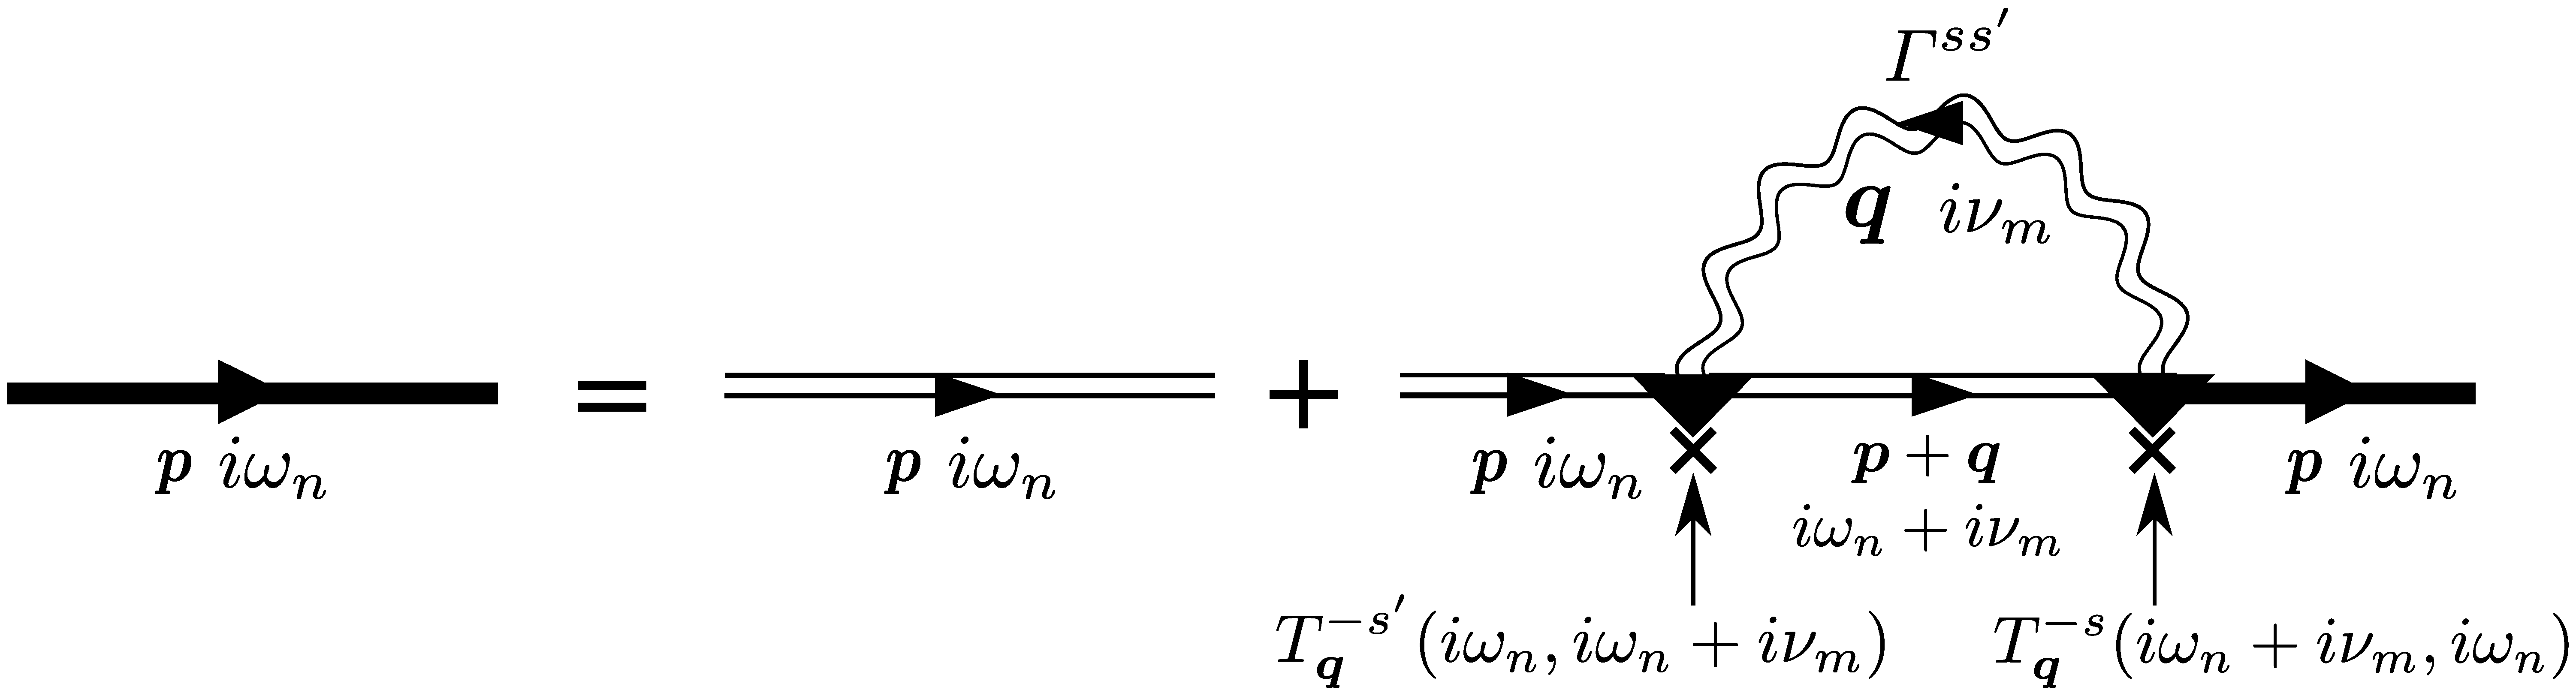
\includegraphics[width=120mm]{eps/belowtc-dyson.eps}
\end{center}
\caption{非磁性不純物を含むフェルミ原子気体の強結合効果に対する $T$ 行列理論のダイソン方程式。太線は 1 粒子グリーン関数 $\bgpom$、二重波線は $\varGamma^{ss'}$ (式 (\ref{eq:append:gam:gam}))、二重実線は BCS-Leggett 理論のグリーン関数 $\bgimppom$, $\times$ 付きの黒三角形は $T^s$ (式 (\ref{eq:append:tma:tsom})) を表す。}
\label{fig:below:dyson:all}
\end{figure}

前節で求めた $\tsom$(式 (\ref{eq:append:asdfasdfasdf}))、$\varGamma^{s,s'}_{\bq}(i \num)$ (式 (\ref{eq:append:asdfjjjjjjj}))を用いて、 非磁性不純物の $T$ 行列理論は図 \ref{fig:below:dyson:all} によって与えられる。図 \ref{fig:below:dyson:all} の自己エネルギーは、
\beq
\bsigpom &= (-1)^{n=1} \frac{1}{\beta}\sumn \sum_{\bp} \sum_{s,s'=\pm} \varGamma^{ss'}_{\bq}(i\num) T^{-s'}_{\bq}(i\omn,i\omn+i\num) \notag\\
&\qquad \times \bggg^{\imp}_{\bp+\bq}(i\omn+i\num) T^{-s}_{-\bq}(i\omn+i\num,i\omn),\label{eq:append:eq:bsigpom}
\eeq
となる。

自己エネルギー(式 (\ref{eq:append:eq:bsigpom}))を、式 (\ref{eq:asdfasdfasdfasdf})、 (\ref{eq:append:asdfjjjjjjj})、 (\ref{eq:append:asdfjjjjjjj})-(\ref{eq:thissection:f:f}) から求め、
\beq
\bgpom= \frac{1}{\left[ \bgimppom\right]^{-1} - \bsigpom},
\eeq
として、 1 粒子グリーン関数を計算することができる。


\clearpage
\section{超流動転移温度以上への書き換え方法}\label{sec:append:rewritetmat}


\begin{figure}[t]
\begin{center}
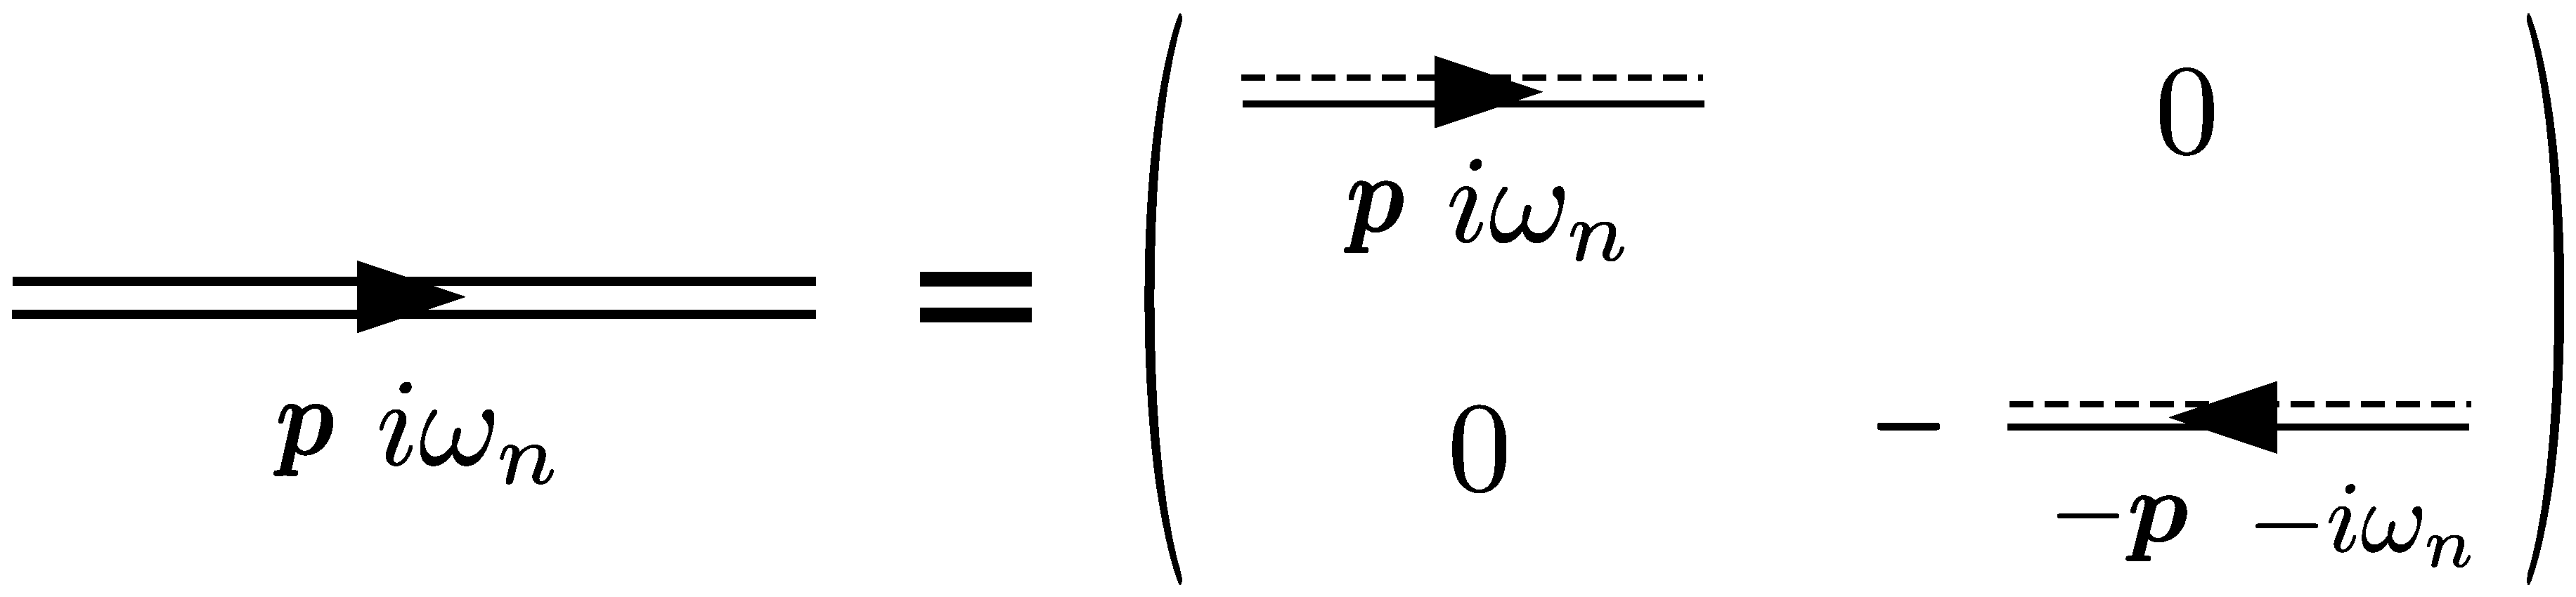
\includegraphics[width=70mm]{eps/rewriting-grenn.eps}
\end{center}
\caption{ 2 成分南部場表示でのグリーン関数の超流動転移温度以上での書き換え。二重実線は南部表示による $2 \times 2$ 行列グリーン関数。波線と実線の二重線は 1 成分表示でのグリーン関数。}
\label{fig:below:dyson:rewrite-grenn}
\end{figure}

超流動転移温度以上では $\del=0$ となるので、図 \ref{fig:below:dyson:rewrite-grenn} のようにグリーン関数の非対角要素がゼロになり、
\beq
\bggg_{\bp}^{\imp}(i\omn) = \begin{pmatrix} G_{\bp\uar}^{\imp}(i\omn) &0\\0&-G^{\imp}_{-\bp\dar}(-i\omn)\end{pmatrix},\label{eq:section:f:h}
\eeq
と 1 成分のグリーン関数に分解できる。

\begin{figure}[t]
\begin{center}
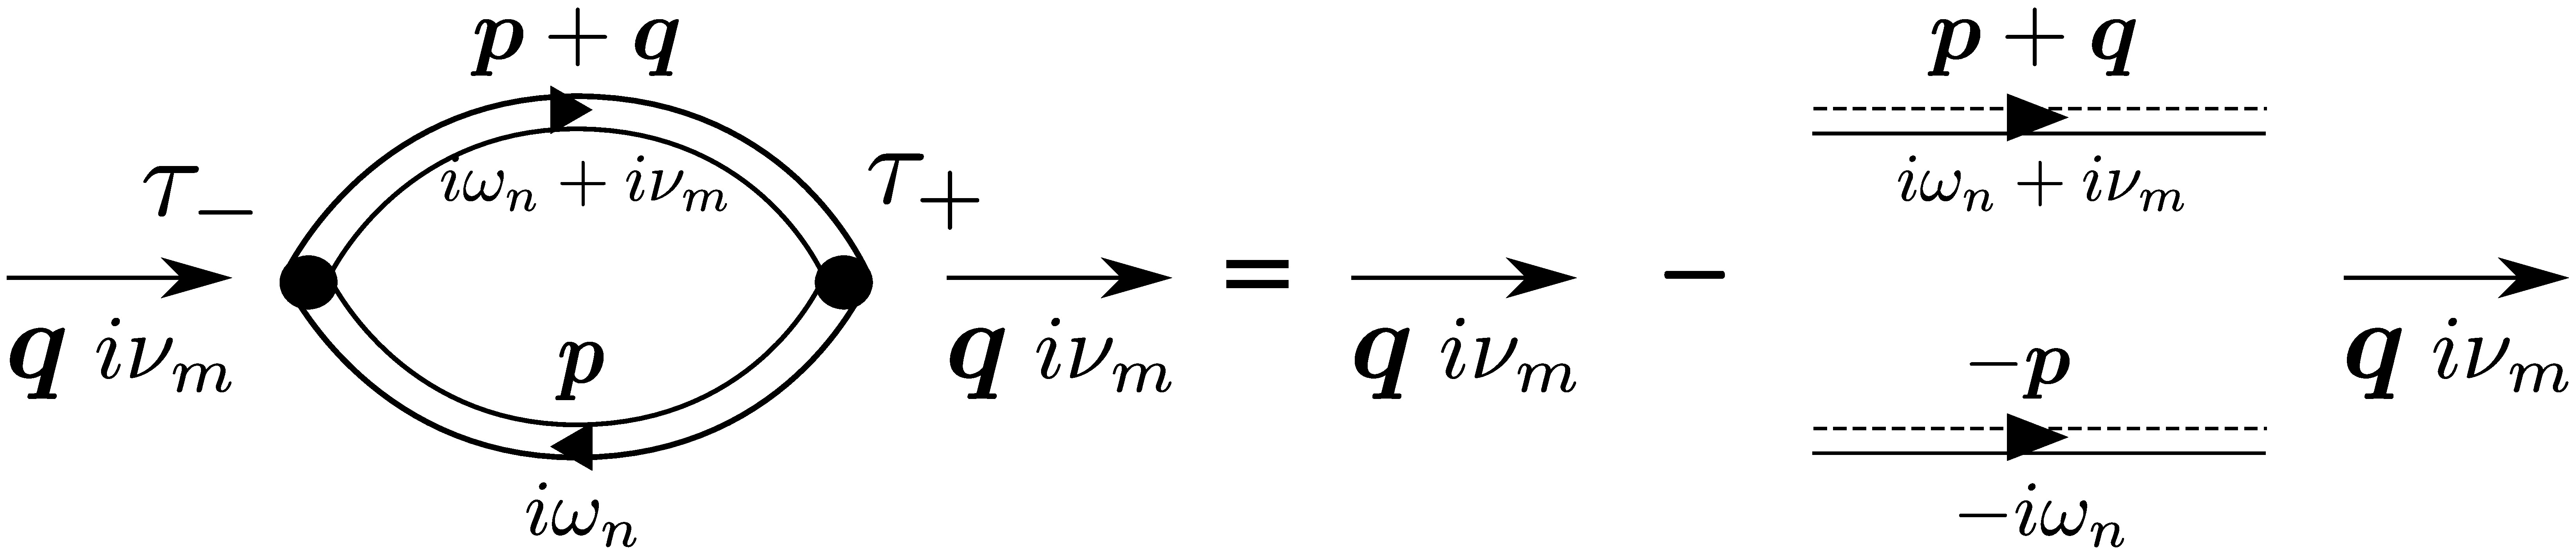
\includegraphics[width=90mm]{eps/rewriting-loop.eps}
\end{center}
\caption{南部表示でのループ構造部分を 1 成分のグリーン関数に書き換える方法。グラフルールにおけるフェルミ粒子線ループから出る左辺のマイナス符号は、右辺では図 \ref{fig:below:dyson:rewrite-grenn} の書き換えからくる符号で表現される。}
\label{fig:below:dyson:rewrite-loop}
\end{figure}

\begin{figure}[t]
\begin{center}
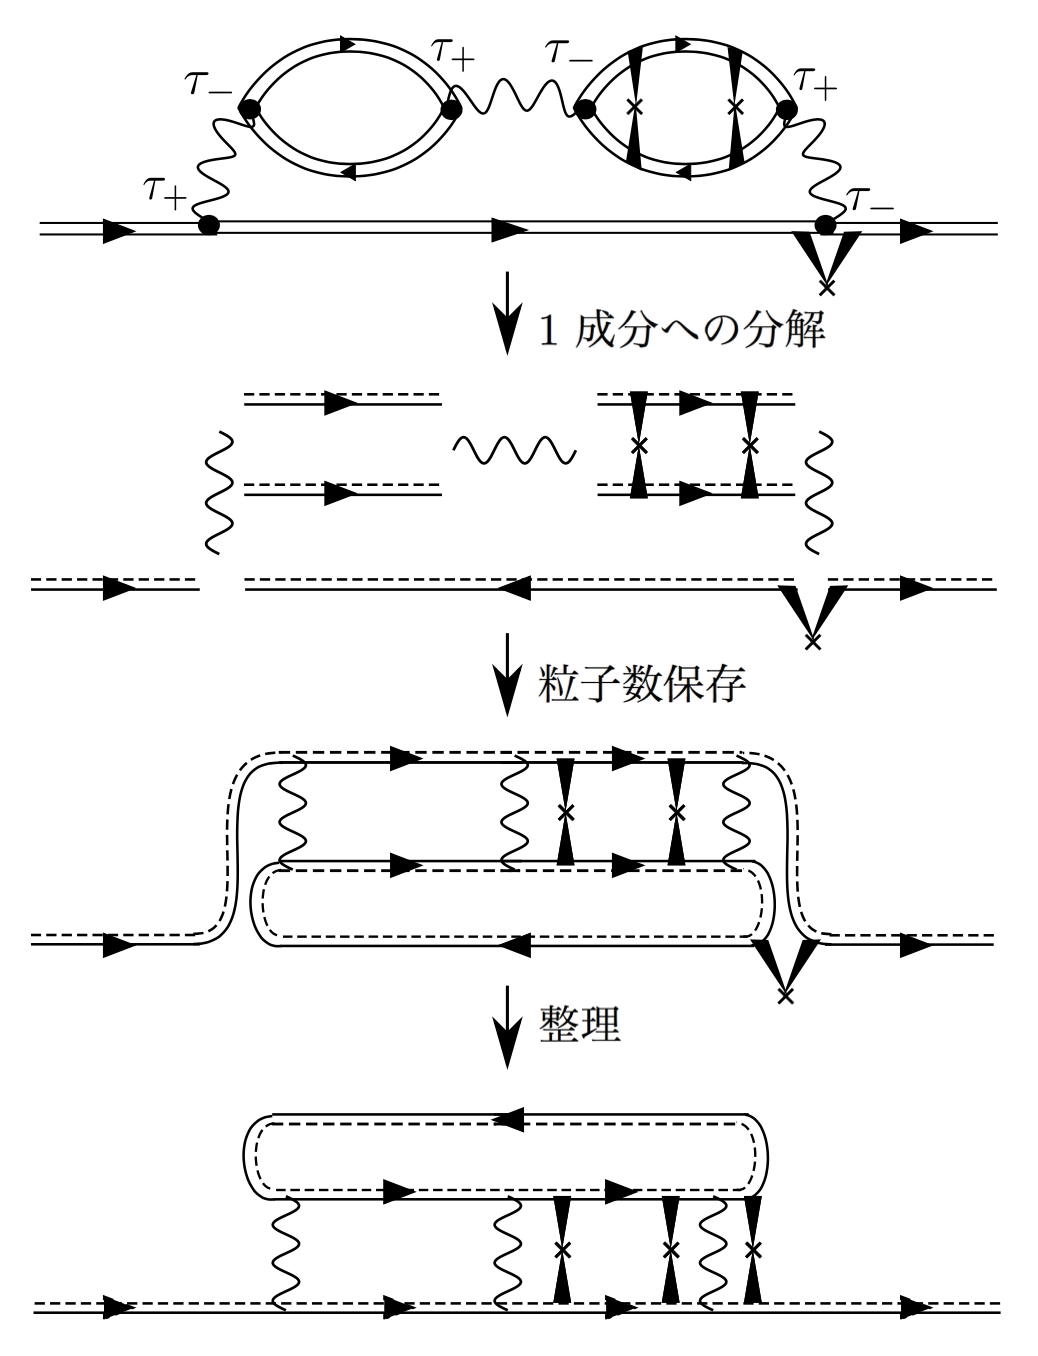
\includegraphics[width=70mm,bb=0 0 519 678]{eps/rewriting.png}
\end{center}
\caption{南部場での行列ダイアグラムの 1 成分のダイアグラムへの書き換え。1 成分グリーン関数に分解するためには、南部表示で $\tau_{\pm}$ が現れる部分で 1 成分表示のグリーン関数の向きが変わるので、一度切り分ける。切り分けたグリーン関数を、一つの直線上で粒子数やスピンが保存するように再度つなぎ直し、トポロジカルに等しいダイアグラムへと整理する。}
\label{fig:below:dyson:rewrite}
\end{figure}

同様に、南部場のループは図 \ref{fig:below:dyson:rewrite-loop} のように 1 成分のダイアグラムへと分解できる。ダイアグラムルールを適用すると、図 \ref{fig:below:dyson:rewrite-loop} の左辺はフェルミオンのループがあるために負符号が出るが、式 (\ref{eq:section:f:h}) のグリーン関数の $(2,2)$ 成分への書き換え時に出てくる負符号によって相殺するので、ループがないダイアグラムへの書き換えができる。

図 \ref{fig:below:dyson:rewrite-grenn} と 図 \ref{fig:below:dyson:rewrite-loop} の書き換え方法を用いて、南部場で書かれた $T$ 行列理論を 1 成分で書かれた $T$ 行列理論へと書き換える方法の一例として図 \ref{fig:below:dyson:rewrite} を記述した。

以上の書き換えを用いれば、\ref{sec:form:tmat} 節で定義した記号を右辺に用いて、
\beq
\bvvtxn &=  \begin{pmatrix} V_{\imp}(i \omn) & 0 \\ 0& -V_{\imp}(-i\omn) \end{pmatrix},\notag\\
T^{+}_{\bq}(i\omn,i\omn+i\num)&=t_q(i\omn,-i\omn-i\num) \tau_+,\notag\\
T^{-}_{\bq}(i\omn,i\omn+i\num)&=t_q(-i\omn,i\omn+i\num) \tau_-,\notag\\
\varPi^{\imp,+-}_{\bq}(i\num) &= -\varPi^{\imp}_{-\bq,\uar}(-i\num),\notag\\
\varPi^{\imp,-+}_{\bq}(i\num) &= -\varPi^{\imp}_{\bq,\dar}(i\num), \notag\\
\varPi^{\imp,++}_{\bq}(i\num) &= \varPi^{\imp,--}_{\bq}(i\num) = 0\notag\\
\varGamma^{+-}_{\bq}(i\num) &= \varGamma_{-\bq\uar}(-i\num), \notag\\
 \varGamma^{-+}_{\bq} (i\num) &= \varGamma_{\bq \dar}(i\num),\notag\\
\varSigma_{\bp}^{11}(i\omn) &= - \varSigma_{\bp\uar}(i\omn), \notag\\
\varSigma_{\bp}^{22}(i \omn) &= - \varSigma_{\bp\dar}(i\omn)
\eeq 
等の関係が示せ、これらを用いることで \ref{sec:form:tmat} 節の定式化に帰着する。

\chapter{状態密度の計算方法}\label{sec:append:dosodosdoododosdosodosda}

1 粒子温度グリーン関数 $\gpom$ を $\omn>0$ に対し、$i\omn\to\omega+i \delta$ と解析接続したものは、遅延グリーン関数,
\beq
G_{\bp}(t) = - i \theta(t) \braket{\left[c_{\bp}(t), c^{\dag}_{\bp}(0)\right]_{+}},
\eeq
をフーリエ変換したものと一致する \cite{zubarev1960}。これを利用すると、 1 粒子スペクトル強度 $A_{\bp}(\omega)$ は、
\beq
A_{\bp}(\omega) = - \frac{1}{ \pi} \im G_{\bp}(i \omn \to \omega + i \delta).
\eeq
のように解析接続された温度グリーン関数の虚部で与えられ、それを運動量 $\bp$ で和を取ることにより 1 粒子状態密度が得られる:
\beq
\rho(\omega) = - \frac{1}{ \pi} \im \sum_{\bp} G_{\bp}(i \omn \to \omega+ i \delta).
\eeq
2 成分南部場で表示した温度グリーン関数を用いる場合、行列要素のうち $(1,1)$ 成分に対し、同様の操作をすることで、粒子の状態密度を計算することができる。尚、本論文では解析接続は Pad\'e 近似により数値的に行う。
